本问求解流程如下：
\begin{figure} [H]
    \centering
    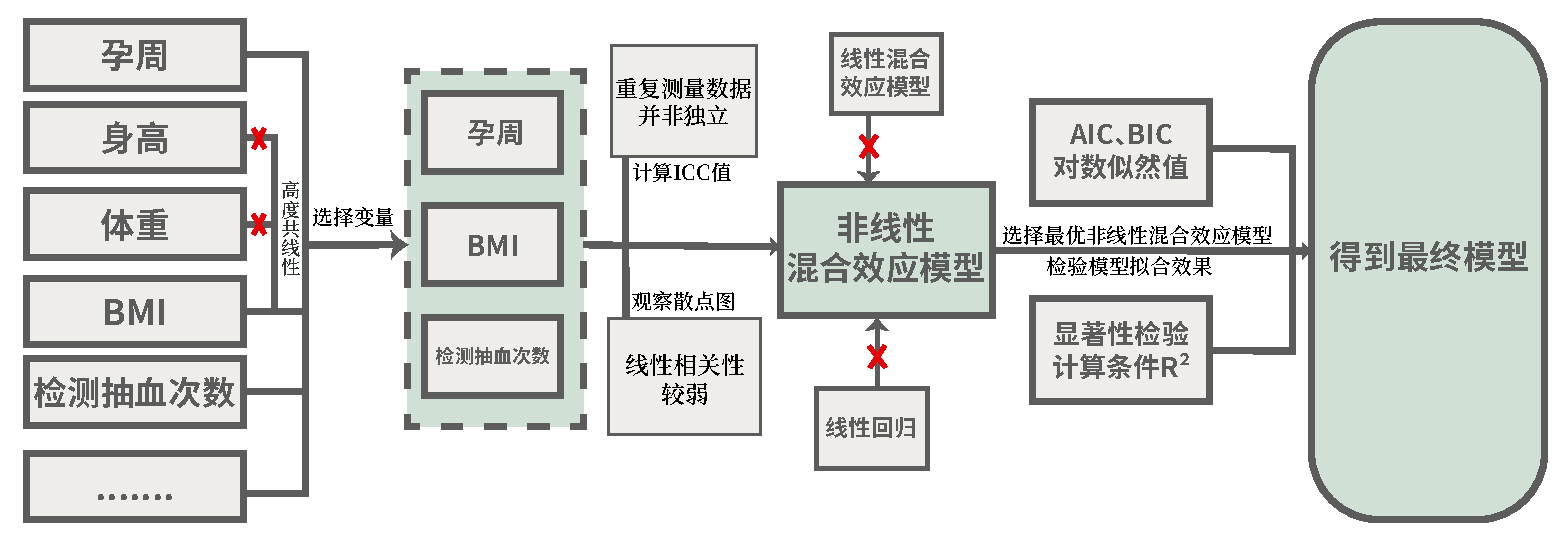
\includegraphics[width=\textwidth]{chapters/Q1/images/问题一的模型建立与求解/问题1流程图.pdf}
    \caption{问题1求解流程图}
    \label{fig:flowchart1}
\end{figure}

\subsection{符号说明}

为便于模型建立，本文对新增符号进行说明，其余符号沿用上文。

\begin{center}
    \begin{tabularx}{0.7\textwidth}{c@{\hspace{1pc}}|@{\hspace{2pc}}>{\centering\arraybackslash}X}
        \Xhline{0.08em}
        符号    & 符号说明               \\
        \Xhline{0.05em}
        $Y_i$ & 第 $i$ 个样本的 Y 染色体浓度 \\
        $c_i$ & 第 $i$ 个样本的检测抽血次数   \\
        \Xhline{0.08em}
    \end{tabularx}
\end{center}

\subsection{多重共线性分析与变量选择}

由于 BMI 可由身高体重得到，本文通过计算方差膨胀因子（VIF）以衡量这几个变量间的多重共线性程度。对于模型中的第 $i$ 个自变量，其 VIF 值的计算公式为：
$$
    \text{VIF}_i = \frac{1}{1 - R_i^2}
$$
其中，$R_i^2$ 是将自变量 $x_i$ 作为因变量，对数据集中所有其他自变量进行线性回归时所得到的决定系数。通常认为，当 $VIF > 10$ 时，模型存在严重的共线性问题。

计算可得，身高、体重与 BMI 三者存在多重共线性（如表 \ref{tab:vif_analysis} 所示，三个变量的 VIF 值均远大于 $10$），因此建模时仅选用 BMI 作为孕妇体型的代表指标。对于其他因素，图 \ref{fig:Y} 展示了多种孕妇因素与 Y 染色体浓度的散点图。

\begin{table}[H]
    \centering
    \caption{孕妇体重、身高与 BMI 的VIF值}
    \label{tab:vif_analysis}
    \begin{tabular}{ccc}
        \toprule
        \textbf{体重 VIF} & \textbf{孕妇BMI VIF} & \textbf{身高 VIF} \\
        \midrule
        360.38          & 224.34             & 109.31          \\
        \bottomrule
    \end{tabular}
\end{table}

\begin{figure} [H]
    \centering
    
\includegraphics[width=0.8\textwidth]{chapters/Q1/images/问题一的模型建立与求解/Y染色体浓度与有关系的变量的散点图.pdf}
    \caption{Y 染色体浓度与有关系的变量的散点图}
    \label{fig:Y}
\end{figure}

考虑到生产次数较多的孕妇与大龄产妇较少，在样本不足的情况下，无法确凿断定这两个因素对 Y 染色体浓度的影响。且随着生产次数的增多，Y 染色体浓度均值仍维持在 $0.08$ 左右，如表 \ref{tab:parity_Y} 所示：

\begin{table}[H]
    \centering
    \caption{按生产次数分组的 Y 染色体浓度均值}
    \label{tab:parity_Y}
    \begin{tabular}{c|cccc}
        \toprule
        \textbf{生产次数}      & 0      & 1      & 2      & 3      \\
        \midrule
        \textbf{Y 染色体浓度均值} & 0.0770 & 0.0759 & 0.0850 & 0.0789 \\
        \bottomrule
    \end{tabular}
\end{table}

若将 $a_i > 35$ 作为大龄产妇标准剔除，剔除前后其均值也几乎维持不变（全体样本：$0.07719$，剔除后：$0.07745$），仅相差 $0.34\%$，与散点图较为符合。因此本文认为：

\begin{itemize}[leftmargin=2em]
    \item 生产次数对 Y 染色体浓度不产生显著影响；
    \item 孕妇年龄对 Y 染色体浓度不产生显著影响；
\end{itemize}

除本文假设外，在一项针对超过两万名孕妇的大样本研究中\cite{zhou2015effects}，专门通过测量 Y 染色体来估算胎儿分数，其采用的模型如下：
\begin{equation}
    \varepsilon_{i,Y} = \frac{cr_{i,Y} - cr'_{i,Y,f}}{cr'_{i,Y,m} - cr'_{i,Y,f}}
    \label{eq:fetal_fraction}
\end{equation}
其中 $\varepsilon_{i,Y}$ 代表样本 $i$ 通过 Y 染色体估算出的胎儿分数。该研究明确指出，胎儿分数（即Y染色体浓度）与男胎母体年龄并无相关性，为本文的假设提供了有力支撑。

数据统计阶段可知，胎儿 Y 染色体浓度与大部分生理指标存在较弱的线性相关性。而由散点图（图 \ref{fig:Y}）可知，孕周、BMI 存在一定的正负相关性。离群散点较多，使用单纯的线性模型拟合效果不足。综合考虑下，本文选用探究\textbf{孕妇 BMI 值、孕周（或孕天数）与检测抽血次数}三个指标与 \textbf{Y 染色体浓度的非线性关系}。

\subsection{重复测量数据的非独立性}

考虑到数据中存在大量针对同一孕妇的重复测量记录，数据观测值之间并非相互独立，如对同一个样本进行多次的测量（如本题中的多次采血），该类数据被称为重复测量数据\cite{feng2020}。其特点是同一研究对象的重复测量值之间是非独立的。并且可能存在由于个体差异引起的相关性。传统的 $t$ 检验与方差分析，都要求数据具有独立性。

此类调查方式在生物医学研究中称为纵向研究。纵向研究与横断面研究有根本的区别。横断面研究是在个体只被观察一次的情况下进行的。然而，纵向研究关注于调查在不同时间上的变化，主要特征是研究对象在一段时间内被重复测量。

查找相关文献发现，混合效应模型（Mixed Effect Model）对同一统计单位进行重复测量或对相关统计单位集群进行测量的情况下有明显作用\cite{gomes2022should}，该模型能够将数据的变异区分为：代表普遍规律的固定效应和代表个体差异的随机效应\cite{gomes2022should}，进而可以得到更准确可靠的参数估计。

为定量验证采用混合效应模型的必要性，需首先计算Y染色体浓度达的组内相关系数（ICC）。ICC用于量化同一组\textbf{测量结果}之间的相关程度，在本题的情境下即同一孕妇的多个Y染色体浓度测量结果，其计算公式如下\cite{yu2022beyond}：
\begin{equation}
    \text{ICC} = \frac{\sigma_b^2}{\sigma_b^2 + \sigma_e^2}
\end{equation}
其中，$\sigma_b^2$ 表示组间方差，即不同孕妇之间的差异；$\sigma_e^2$ 表示组内方差，即同一孕妇的波动。ICC 的取值范围为 $0$ 到 $1$，如果 $ICC = 0$，则数据可视为不相关；如果 $ICC = 1$，则每个聚类中的所有观测值都完全相关。

Terry K. Koo 提出了检验 ICC 值的标准\cite{koo2016guideline}，具体如下：

\begin{itemize}[leftmargin=2em]
    \item $ICC < 0.5$，表示测量结果之间的相关性较差(原文为 Poor)；
    \item $0.5 \leq ICC < 0.75$，表示测量结果之间的相关性中等(原文为 Moderate)；
    \item $0.75 \leq ICC < 0.9$，表示测量结果之间的相关性良好(原文为 Good)；
    \item $ICC \geq 0.9$，表示测量结果之间的相关性极好(原文为 Excellent)。
\end{itemize}

\subsection{挑选最优非线性混合效应模型}

使用Python的 statsmodels 库对数据进行分析，计算得到 $ICC = 0.5984$，这说明同一孕妇的Y染色体浓度测量结果之间存在中等程度的相关性，所以混合效应模型在本题中是适用的。普通的非线性回归模型由于存在变量之间相互独立的假设，在本题中并不适用。因此，本文建立如下可能的非线性混合效应模型：
$$
    \begin{cases}
        Y = \beta_0 + \beta_1 w + \beta_2 w^2 + \beta_3 BMI + \beta_4 c                          & (a) \\
        Y = \beta_0 + \beta_1 w + \beta_2 w^2 + \beta_3 BMI + \beta_4 BMI^2 + \beta_5 c          & (b) \\
        Y = \beta_0 + \beta_1 w + \beta_2 w^2 + \beta_3 BMI + \beta_4 c + \beta_5 c^2            & (c) \\
        Y = \beta_0 + \beta_1 w + \beta_2 w^2 + \beta_3 BMI + \beta_4 c + \beta_5 (BMI \times w) & (d)
    \end{cases}
$$
其中，$Y$ 表示 Y 染色体浓度，$w$ 表示孕周数，$BMI$ 表示孕妇 BMI 值，$c$ 表示检测抽血次数，$\beta_i (i=0,1,2,\ldots)$ 为待估计的模型参数。

为了选择最优模型，本文使用赤池信息量准则（AIC）和贝叶斯信息量准则（BIC）作为模型评价指标。AIC和BIC均考虑了模型的拟合优度和复杂度，其值越小代表模型在解释数据和避免过拟合之间达到了更好的平衡。
AIC和BIC的计算公式如下：
\begin{numcases}
    \text{AIC} = 2k - 2\ln(L) \\
    \text{BIC} = k\ln(n) - 2\ln(L)
\end{numcases}

其中，$k$ 为模型参数的数量，$L$ 为模型的最大似然估计值，$n$ 为样本数量。计算结果如表 \ref{tab:model_comparison} 所示：

\begin{table}[H]
    \centering
    \caption{不同模型的比较结果}
    \label{tab:model_comparison}
    \begin{tabular}{lccc}
        \toprule
        \textbf{模型名称} & \textbf{AIC} & \textbf{BIC} & \textbf{对数似然值} \\
        \midrule
        模型\textit{a} & -5117.046702 & -5082.166662 & 2565.523351    \\
        模型\textit{c} & -5106.499492 & -5066.636590 & 2561.249746    \\
        模型\textit{b} & -5098.236333 & -5058.373431 & 2557.118166    \\
        模型\textit{d} & -5097.598194 & -5057.735292 & 2556.799097    \\
        \bottomrule
    \end{tabular}
\end{table}

由表 \ref{tab:model_comparison} 可知，模型 $a$ 的 AIC 和 BIC 值均为最小，且对数似然值最大，说明该模型在解释数据和避免过拟合之间达到了更好的平衡。因此，本文选择模型 $a$ 作为最终的非线性混合效应模型。
对模型$a$进行拟合，得到如下结果：

\begin{table}[H]
    \centering
    \caption{模型的拟合结果}
    \label{tab:model_fit}
    \begin{tabular}{l c c c c c c}
        \toprule
                                        & \textbf{Coef.} & \textbf{Std.Err.} & \textbf{z} & \textbf{P>|z|} & \multicolumn{2}{c}{\textbf{[0.025 0.975]}}          \\
        \midrule
        \textbf{Intercept}              & 0.218          & 0.020             & 10.705     & 0.000          & 0.178                                      & 0.258  \\
        \textbf{孕周}                     & -0.012         & 0.002             & -7.880     & 0.000          & -0.015                                     & -0.009 \\
        \textbf{孕周 \textsuperscript{2}} & 0.000          & 0.000             & 8.598      & 0.000          & 0.000                                      & 0.000  \\
        \textbf{孕妇BMI}                  & -0.002         & 0.000             & -4.290     & 0.000          & -0.003                                     & -0.001 \\
        \textbf{检测抽血次数}                 & 0.012          & 0.001             & 10.936     & 0.000          & 0.010                                      & 0.014  \\
        \bottomrule
    \end{tabular}
\end{table}

由于表 \ref{tab:model_fit} 中的数据会进行四舍五入，导致部分数字显示为 $0.000$。为检验\textbf{显著性水平}，Statsmodels库在构建此模型时会同步进行沃尔德检验，其核心思想在于评估参数的点估计值与其标准误差的比值：对于模型中的每一个参数 $\beta_j$，本文首先设立原假设 $H_0: \beta_j=0$，即该变量对因变量没有影响。随后计算 $z$ 统计量：
\begin{equation}
    z = \frac{\hat{\beta}_j}{\text{SE}(\hat{\beta}_j)}
\end{equation}
其中，$\hat{\beta}_j$ 是参数 $\beta_j$ 的最大似然估计值，$\text{SE}(\hat{\beta}_j)$ 是其对应的标准误差。在原假设成立的条件下，该 $z$ 统计量近似服从标准正态分布。

基于此，本文的详细检验结果已在表 \ref{tab:pvalues} 中呈现，所有变量的 $p$ 值均远小于 0.05，证明了其高度的统计显著性。

\begin{table}[H]
    \centering
    \caption{回归系数表}
    \label{tab:coefficients}
    \begin{tabular}{lccccc}
        \toprule
        \textbf{变量}         & \textbf{Intercept} & \textbf{孕周} & \textbf{孕周$^2$} & \textbf{孕妇BMI} & \textbf{检测抽血次数} \\
        \midrule
        \textbf{系数 (Coef.)} & 0.218290           & -0.011993   & 0.000326        & -0.002045      & 0.012028        \\
        \bottomrule
    \end{tabular}
\end{table}

\begin{table}[H]
    \centering
    \caption{显著性水平表}
    \label{tab:pvalues}
    \begin{tabular}{lccccc}
        \toprule
        \textbf{变量}         & \textbf{Intercept} & \textbf{孕周}  & \textbf{孕周$^2$} & \textbf{孕妇BMI} & \textbf{检测抽血次数} \\
        \midrule
        \textbf{p值 (P>|z|)} & 9.601115e-27       & 3.262814e-15 & 8.078243e-18    & 1.784269e-05   & 7.727184e-28    \\
        \bottomrule
    \end{tabular}
\end{table}

由表 \ref{tab:coefficients} 可知，在混合效应模型中，各变量的系数均不为零，孕周与孕妇BMI与Y染色体浓度呈负相关，而孕周平方与检测抽血次数则与Y染色体浓度呈正相关。由表 \ref{tab:pvalues} 可知，所有变量的 $p$ 值均远小于 $0.05$，说明在统计学上均显著影响 Y 染色体浓度，通过显著性检验。
此前的研究已普遍发现：胎儿 DNA 浓度随孕龄增加而增加，随孕妇体重增加而减少。因此，本文构建的最终的非线性混合效应模型为：
\begin{equation}
    Y = 0.218290 - 0.011993 w + 0.000326 w^2 - 0.002045 BMI + 0.012028 c \label{eq:final_model}
\end{equation}
其中，$Y$ 表示 Y 染色体浓度，$w$ 为孕周数，$c$ 表示检测抽血次数。

从统计学角度看，文献中的发现也与本模型的变量显著性结论一致。研究明确指出，孕周与 Y 染色体浓度的相关性 ($P<.001$) 以及孕妇 BMI 与其的相关性 ($P<.001$) 均达到了统计学上的高度显著水平\cite{zhou2015effects}。这表明将孕周、孕周的二次方以及孕妇 BMI 纳入模型是合理且必要的。

本文还对模型的条件 $R^2$ 值进行了计算，以评估模型的解释力。条件 $R^2$ 值考虑了固定效应和随机效应的贡献，其计算公式为：
\begin{equation}
    R^2_c = \frac{\sigma_f^2 + \sigma_r^2}{\sigma_f^2 + \sigma_r^2 + \sigma_e^2}
    \label{eq:conditional_r2}
\end{equation}
其中，$\sigma_f^2$ 表示固定效应的方差，$\sigma_r^2$ 表示随机效应的方差，$\sigma_e^2$ 表示残差的方差。

计算得到模型的条件 $R^2$ 值为 $0.7664$，说明模型能够解释约 $76.64\%$ 的 Y 染色体浓度的变异。本文也将模型的拟合效果可视化，如图 \ref{fig:model_fit} 所示：
\begin{figure}[H]
    \centering
    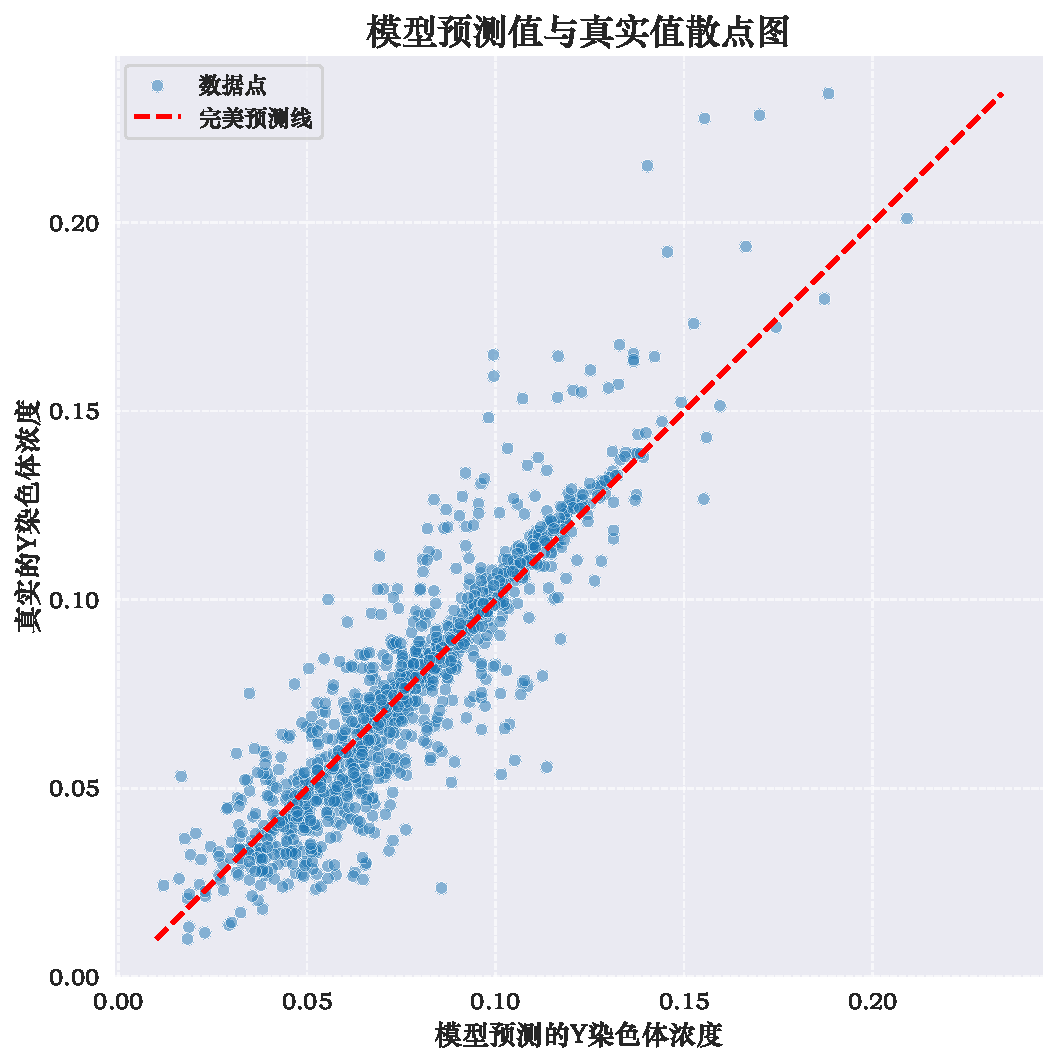
\includegraphics[width=0.6\textwidth]{chapters/Q1/images/问题一的模型建立与求解/预测值与真实值.pdf}
    \caption{模型的拟合效果图}
    \label{fig:model_fit}
\end{figure}

综上，对于问题一，本文综合考虑孕妇 BMI 值、孕周与检测抽血次数三个指标，建立了一个非线性混合效应模型来描述这些因素与 Y 染色体浓度之间的关系。通过模型选择和评估，最终确定了模型 $a$ 作为最优模型，拟合出的模型系数也呈现出极强的显著性。此外，模型的条件 $R^2$ 值为 $0.7664$，说明该模型具有较强的解释力，能够较好地反映孕妇相关因素对 Y 染色体浓度的影响。
